% Options for packages loaded elsewhere
\PassOptionsToPackage{unicode}{hyperref}
\PassOptionsToPackage{hyphens}{url}
\PassOptionsToPackage{dvipsnames,svgnames*,x11names*}{xcolor}
%
\documentclass[
  12pt,
]{article}
\usepackage{lmodern}
\usepackage{amssymb,amsmath}
\usepackage{ifxetex,ifluatex}
\ifnum 0\ifxetex 1\fi\ifluatex 1\fi=0 % if pdftex
  \usepackage[T1]{fontenc}
  \usepackage[utf8]{inputenc}
  \usepackage{textcomp} % provide euro and other symbols
\else % if luatex or xetex
  \usepackage{unicode-math}
  \defaultfontfeatures{Scale=MatchLowercase}
  \defaultfontfeatures[\rmfamily]{Ligatures=TeX,Scale=1}
\fi
% Use upquote if available, for straight quotes in verbatim environments
\IfFileExists{upquote.sty}{\usepackage{upquote}}{}
\IfFileExists{microtype.sty}{% use microtype if available
  \usepackage[]{microtype}
  \UseMicrotypeSet[protrusion]{basicmath} % disable protrusion for tt fonts
}{}
\makeatletter
\@ifundefined{KOMAClassName}{% if non-KOMA class
  \IfFileExists{parskip.sty}{%
    \usepackage{parskip}
  }{% else
    \setlength{\parindent}{0pt}
    \setlength{\parskip}{6pt plus 2pt minus 1pt}}
}{% if KOMA class
  \KOMAoptions{parskip=half}}
\makeatother
\usepackage{xcolor}
\IfFileExists{xurl.sty}{\usepackage{xurl}}{} % add URL line breaks if available
\IfFileExists{bookmark.sty}{\usepackage{bookmark}}{\usepackage{hyperref}}
\hypersetup{
  pdftitle={Assignment ASR},
  pdfauthor={Frederic Denker},
  colorlinks=true,
  linkcolor=Maroon,
  filecolor=Maroon,
  citecolor=Blue,
  urlcolor=blue,
  pdfcreator={LaTeX via pandoc}}
\urlstyle{same} % disable monospaced font for URLs
\usepackage[margin=2.5cm]{geometry}
\usepackage{graphicx,grffile}
\makeatletter
\def\maxwidth{\ifdim\Gin@nat@width>\linewidth\linewidth\else\Gin@nat@width\fi}
\def\maxheight{\ifdim\Gin@nat@height>\textheight\textheight\else\Gin@nat@height\fi}
\makeatother
% Scale images if necessary, so that they will not overflow the page
% margins by default, and it is still possible to overwrite the defaults
% using explicit options in \includegraphics[width, height, ...]{}
\setkeys{Gin}{width=\maxwidth,height=\maxheight,keepaspectratio}
% Set default figure placement to htbp
\makeatletter
\def\fps@figure{htbp}
\makeatother
\setlength{\emergencystretch}{3em} % prevent overfull lines
\providecommand{\tightlist}{%
  \setlength{\itemsep}{0pt}\setlength{\parskip}{0pt}}
\setcounter{secnumdepth}{-\maxdimen} % remove section numbering
\usepackage{dcolumn}
\usepackage{setspace}
\doublespacing
\usepackage[utf8]{inputenc}
\usepackage{float}
\usepackage{xcolor}
\usepackage{lipsum}

\title{Assignment ASR}
\author{Frederic Denker}
\date{Juni 01, 2020}

\begin{document}
\maketitle

\hypertarget{research-summary}{%
\subsection{Research Summary:}\label{research-summary}}

\hypertarget{managerial-summary}{%
\subsection{Managerial Summary}\label{managerial-summary}}

\hypertarget{keywords}{%
\subsection{Keywords}\label{keywords}}

patent citation, utility models, innovation policy

\newpage

\hypertarget{introduction}{%
\subsection{Introduction}\label{introduction}}

Innovation is accredited with much of the improvements in levels of
human welfare. However, in order to make sure that this trend continues,
it must be made sure that the incentives to innovate stay strong.
Special attention needs to be paid on how government policy can maintain
these incentives in times in which the pace of technological and
societal change is accelerating (SAUCE).

This paper will examine one of the mechanism that was first introduced
by the German government in 1891: the utility model (Goldstein and
Straus 2009). Utility models will be introduced in more detail below
TEST . It was soon used as a model legislative structure in countries
like Japan, which introduced it into law in 1905 with much of the same
conditions as the German one (Goldstein and Straus 2009). In the
following years many developing and developed countries have introduced
similar legislation (Prud'homme 2014). However, there has been little to
none quantitative assessment of the usefulness of these Utility models
in contrast to the more studied patents.

This research is especially relevant as several countries such as the
People's Republic of China have modelled their IP system after the
German one without rigorous examinations of its effects (Prud'homme
2014).

However, the literature on the real-world usage of these utility models
in contrast to the more widespread patents is quite scarce. This paper
will use citations in US patent applications as a means to better
understand the usefullness of different types of IP after their
application.

The research question therefore is:

How do utility models differentiate in their use to traditional
patenting?

\hypertarget{theoretical-background}{%
\subsection{Theoretical Background}\label{theoretical-background}}

The only incentive scheme for innovation introduced in the last 400
years (Scotchmer 2006) and the one that is most widely used today is
intellectual property (IP). Without IP the benefits of creating new
knowledge do not necessarily benefit the inventor and there is little
incentive to invest in innovation on a large-scale. Therefore, the
incentive of the single entrepreneur is to wait for innovation to happen
through the investment of others in order to then copy it with minimal
costs attached. This logic would inherently lead to low investment /
innovation levels (Aghion et al. 2005) and a situation comparable to the
dominant strategy in a prisoners dilemma. IP such as patents or
trademarks are therefore necessary because they enable the appropriation
of the benefits of an investment by those that invested in it when the
benefits were still uncertain.

A substantial amount of research has been conducted about the
theoretical implications of the patent system (Scotchmer, 2004), there
is, however, a glaring lack of quantitative research that comparatively
evaluates the actual performance of different IP mechanisms. The goal of
the paper is to address this gap in research by using the ``revealed
preferences'' of hundreds of thousands of different inventors by
analyzing patent applications. This paper specifically uses citations
used in American patents applications (of foreign IP) to better
understand the usefulness of different types of IP. American patent
applications were used as a starting point due to data availability
reasons and the high amount of basic research on the US Patent system.

However, while US patent citations are the base of analysis, the focus
of this paper itsself will be on a specific differentiation of the
German patent system that is not present in the US but that shows in the
frequency and timing of citations to German IP in American patent
applications. The specialities of the patenting system in Germany that
lend itsself for a deeper analysis of the value created through IP is
duality of the patenting and utility model system. As mentioned
previously, utility models work similarly as a patent in most aspects,
but differentiate themselves in some of the details: they are only valid
for up to 10 years (in contrast to patents, which are valid up to 20
years) and there are not applied for, but simply registered (Königer
2016). Therefore, utility models are not examined by an official of the
German Patent and Trademark office before they are published. This gives
them less validity in court, but ideally speeds up the process from
ideation to registered IP while minimizing the costs. It therefore seems
intuitive that these types of IP are usefull in two cases: When
innovation is incremental a utility model can be used to save money and
if the pace of technological innovation is increasing it might be handy
to use utility models to quickly expand the IP portfolio\footnote{Especially
  as utility model applications count as priority filing dates.}
(Königer 2016).

Having established that intellectual property protection is important,
this paper will now evaluate the effectiveness of utility models vs
patents.

Patents give the inventor the monopoly right to sue for infringement
other companies that are violating the IP\footnote{Or to be precise:
  Patents give inventors (in the US, but near identical law applies in
  Germany) the ``\emph{right to sue for infringement anyone who makes,
  uses, sells, or offers the invention in the country where the patent
  has been issued, or imports or offers to import the invention into
  that country}'' (35 U.S.C. § 194)}. While this gives the inventors the
possibility monetize the fruits of his investment, it also creates
inefficiencies in the form of deadweight loss due to the use of
monopolistic power. It is, therefore, essential to balance the incentive
with the negative impact of deadweight loss (Nordhaus 1969).

Nordhaus shows that there exists such a thing as the equilibrium IP
length which minimizes deadweight loss and therefore maximizes the
welfare for all (Nordhaus 1969). However, applicants of IP have
incentives to not reveal the true value and costs of the invention.
These informations are, however, needed to determine the correct length
of protection for the invention. One of the ways which can help
policymakers tackle this problem is to allow for differentiation in the
IP instruments with the goal to get the applicant to reveal the true
value of the invention (at least the true value according to the
applicant).

\hypertarget{what-are-utility-models-and-why-are-they-different}{%
\subsection{What are utility models and why are they
different?}\label{what-are-utility-models-and-why-are-they-different}}

Here utility models come into play which give similar but more limited
rights as a patent. As mentioned in the introduction, they are only
valid for 10 and not 20 years and are not examined by an official of the
German Patent and Trademark office. Due to this, it is expected that
firms decide to use utility models for incremental innovation while
using traditional patents for radical innovation (Beneito 2006).

One way to measure this is by examining patent citations. A patent
citations means that either the applicant or the examiner believed that
the cited patent which becomes ``prior art'' has relevance for citing
patent application. Patent citations are very common objects of
quantitative analysis due to a number of reasons discussed below and are
used for measuring technological quality, diffusion of information and
many other innovation metrics (Karki 1997). The important information
that is used in the context of this analysis is that when a patent
applications cites prior art, it indicates that the patent / utility
model still have relevance. This may sound obvious to the reader, it is
however, an assumption.

Coming back to the utility models, on would therefore assume that
citations of utility models drop off sharply after the 10 year mark.
Utility models that are cited after they become invalid fall into a one
of three categories: The first case, and the one that will be assumed to
be the most common, is that the original inventor did not use the
correct type of IP as the invention seems to be still relevant. The
second case is that patatents and utility models are cited which are no
longer relevant, but the applicant was the opinion that citing it would
benefit the patent application (CHANGE THIS SENTENCE). Lastly, there is
a third case which can lead to later citations: uncertainty. (HIER NOCH
WAS )

will be shown to not drive the citations after ten year. This is the
under the assumption of perfect information of the values of an
invention one should protect its invention through a patent. However,
this, of course, is a strong assumption and the more realistic case is
that citations to utility models after ten years are also not unlikely.
One would still assume, however, that citations of utility models drop
off significantly earlier than citations of patents (most probably after
10 years)

Furthermore, the literature on patent citations also brings up the
hypothesis that examiners often cite older patent in their examination
of the patent than the applicants themselves (Jaffe, Trajtenberg, and
Fogarty 2000). This too will be tested in this paper and will be
combined with the earlier question on the predicitive power of different
types of IP for the mean citiation time.

\hypertarget{data-and-methods}{%
\subsection{Data and Methods}\label{data-and-methods}}

\hypertarget{description-of-data-sources}{%
\subsubsection{Description of data
sources}\label{description-of-data-sources}}

Due to the niche nature of this topic, no adequate completed dataset is
publically available. Therefore the data was sourced from three
different sources\footnote{These sources and their merging will be
  explained in detail in the appendix 1.} and then joined:

Firstly, data on which US patents cited which German patents/utility
models can be retrieved from the
\href{https://www.patentsview.org/download/}{``Patentsview additional
download page''}. On the same webpage information on these US patents
can be retrieved.

Additional information on the cited German patents/utility models such
as the application date and the kind of IP is needed for the analysis.
For this the
\href{https://www.epo.org/searching-for-patents/data/web-services/ops.html\#tab-1}{Open
Patent Services API} of the European Patent Office was used.

The advantage of patent data is that every entry in the dataset (at
least the patents) was carefully examined by Patent Office Officials
which leads to a very high internal validity of the later analyses
(SAUCE). Additionally, in order to create the highest level of external
validity possible, all citations on American patents from 1976 (the
start of the full text database of the USPTO) until the end of 2019 were
included in the analysis. This gives the analysis the unique opportunity
to (at least for the last forty years) have a complete picture of the
actual patenting processing. There are of

In total 759575 American patents citing 709649 German patents/utility
models are in the dataset. Due to the fact that the citations have an
m:n relationship, a total of 1712799 citations are the basis for further
analyses. There was a total of XXXX patents for which information was
not publically available.

\hypertarget{operationalization}{%
\subsubsection{Operationalization}\label{operationalization}}

The final dataset represents a n:m table for which the year difference
between the American patent application date and the German
patent/utility model patent publication date is calculated. It is
important to note that while most year differences are positive -
meaning that the German patent was published before the American was
applied for - some can be negative. This is a result of rare cases in
which a patent application cites a German patent that was not yet
published.

Additionally, data on who added the patent citation (applicant, examiner
or others) to the application and which kind of IP was cited is also
part of the dataset and will be used in the analysis

\hypertarget{research-approach}{%
\subsubsection{Research approach}\label{research-approach}}

Firstly an overview over the data will be provided in the form of a
summary table and two distributional graphs. In order to be able to
address the research question and the hypothesis more analytically, a
number of regressions will be presented. The regressions will include a
number of common controls for patent citation analysis which should show
``stability'' of the estimator with more independent variables.

\hypertarget{results}{%
\subsection{Results}\label{results}}

\hypertarget{descriptive-statistics}{%
\subsubsection{Descriptive statistics}\label{descriptive-statistics}}

Starting with the descriptive statistics, a summary table of the main
variables is presented below. Firstly, it important to aknowledge that
there is a much higher number of patent citation (\textasciitilde95 \%)
that are cited than utility model citations (\textasciitilde5 \%). This
is best seen when looking at the mean of the ``Patent Dummy''. While
this partly mirrors the higher amount of patent applications than
utility model applications, the descrepancy in the relationship is a lot
higher for the number of citations (HIER NOCH DATEN DAZUHOLEN?).

\begin{table}[!htbp] \centering 
  \caption{} 
  \label{} 
\small 
\begin{tabular}{@{\extracolsep{5pt}}lccccccc} 
\\[-1.8ex]\hline 
\hline \\[-1.8ex] 
Statistic & \multicolumn{1}{c}{N} & \multicolumn{1}{c}{Mean} & \multicolumn{1}{c}{St. Dev.} & \multicolumn{1}{c}{Min} & \multicolumn{1}{c}{Pctl(25)} & \multicolumn{1}{c}{Pctl(75)} & \multicolumn{1}{c}{Max} \\ 
\hline \\[-1.8ex] 
Patent Dummy & 1,712,799 & 1.087 & 0.282 & 0 & 1 & 1 & 2 \\ 
Year of the US patent & 1,712,799 & 2,003.816 & 10.091 & 1,878 & 1,998 & 2,012 & 2,019 \\ 
Year of the German Patent & 1,712,799 & 1,990.266 & 15.905 & 1,879 & 1,980 & 2,002 & 2,020 \\ 
Year difference & 1,712,799 & 13.572 & 13.814 & $-$99.506 & 4.030 & 18.830 & 136.742 \\ 
\hline \\[-1.8ex] 
\end{tabular} 
\end{table}

Furthermore, in order vizualize the distribution of this graphic shows
the distribution of the associated years for both American and German
patents\footnote{It is important to note that the summary table is based
  on the n:m table which means that the US patents and the German IPs
  can be counted multiple times. This is not the case for the graph
  which counts every IP only once}.

\begin{verbatim}
## Warning: Removed 84 row(s) containing missing values (geom_path).
\end{verbatim}

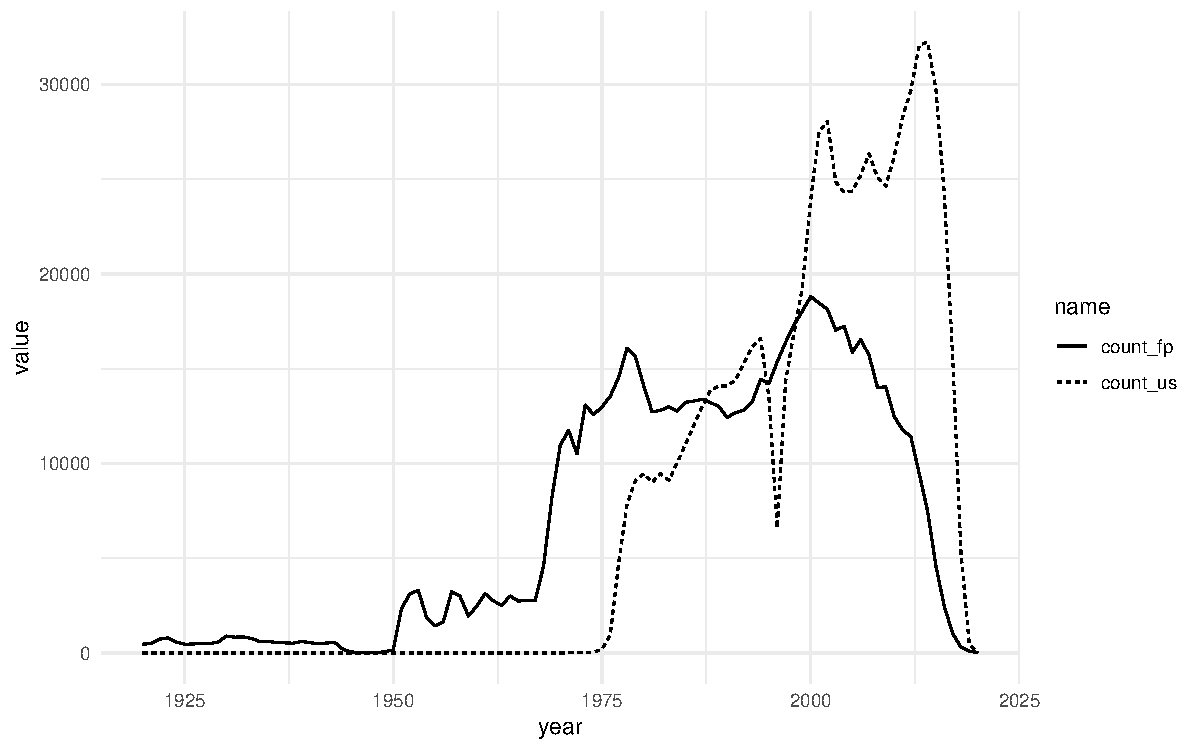
\includegraphics{ASR_Hausarbeit_files/figure-latex/graph_year_patents-1.pdf}

Lastly, in order to create comparability between the two groups, a
density plot is used to visualize the distribution of patent citations.

\begin{verbatim}
## Warning: Removed 41462 rows containing non-finite values (stat_density).
\end{verbatim}

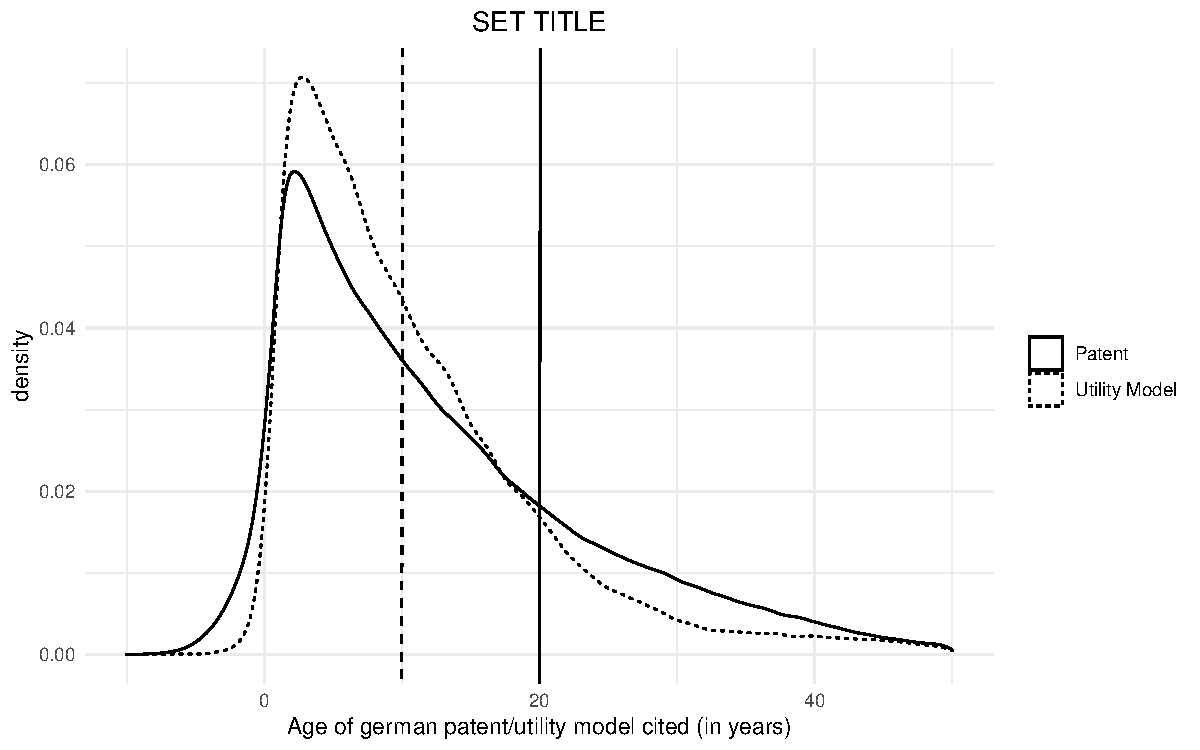
\includegraphics{ASR_Hausarbeit_files/figure-latex/graph_density-1.pdf}

This shows that the relative proportion of utility models and patents
cited by US patents. The most important finding is that the utility
model curve has a higher Kurtosis and seems to have a smaller age
average. However, what is surprising is that utility models are
relatively more cited both at the 10 and 20 year mark. This is confirmed
by the fact that only 24\% of the patent citations are after the patents
expiration while 43\% of the utility model citations are after their
expiration.

These graphical findings can be confirmed by evaluating the regression
results of the \(Table~2\) below:

\begin{table}[h!] \centering 
  \caption{Regression Results} 
  \label{} 
\begin{tabular}{@{\extracolsep{5pt}}lD{.}{.}{-3} D{.}{.}{-3} D{.}{.}{-3} D{.}{.}{-3} } 
\\[-1.8ex]\hline 
\hline \\[-1.8ex] 
 & \multicolumn{4}{c}{\textit{Dependent variable:}} \\ 
\cline{2-5} 
\\[-1.8ex] & \multicolumn{4}{c}{Time difference} \\ 
\\[-1.8ex] & \multicolumn{1}{c}{(1)} & \multicolumn{1}{c}{(2)} & \multicolumn{1}{c}{(3)} & \multicolumn{1}{c}{(4)}\\ 
\hline \\[-1.8ex] 
 Constant & 13.815^{***} & 13.770^{***} & 13.757^{***} & -400.686^{***} \\ 
  & (0.011) & (0.011) & (0.011) & (2.093) \\ 
  Utility model & -2.779^{***} & -2.775^{***} & -2.634^{***} & -3.630^{***} \\ 
  & (0.037) & (0.037) & (0.038) & (0.038) \\ 
  Cited by Examiner &  & 1.138^{***} & 1.450^{***} & 0.531^{***} \\ 
  &  & (0.054) & (0.056) & (0.056) \\ 
  Cited by Examiner | Utility Model &  &  & -3.927^{***} & -3.373^{***} \\ 
  &  &  & (0.200) & (0.198) \\ 
  US patent app. year &  &  &  & 0.207^{***} \\ 
  &  &  &  & (0.001) \\ 
 \hline \\[-1.8ex] 
Observations & \multicolumn{1}{c}{1,712,799} & \multicolumn{1}{c}{1,712,799} & \multicolumn{1}{c}{1,712,799} & \multicolumn{1}{c}{1,712,799} \\ 
\hline 
\hline \\[-1.8ex] 
\textit{Note:}  & \multicolumn{4}{r}{$^{*}$p$<$0.1; $^{**}$p$<$0.05; $^{***}$p$<$0.01} \\ 
\end{tabular} 
\end{table}

For these regressions,a Breusch-Pagan test of linear heteroscedasticity
showed clear heteroscedasticity in the model (See appendix XXXX).
Therefore, the regressions will be run with clustered standard errors.

This regression serves as a statistical confirmation that Utility Models
are on average ceteris paribus cited earlier than Patents. This can be
seen as a hint that utility models are used for incremental innovation
that becomes less useful earlier on.

Furthermore, the third regression give some more insight into what
examiners and applicants cite\footnote{In this regression, NAs and some
  of the categories were excluded from the analysis as they are not
  relevant for this analysis.}. As the goal to examine the actual
decisionmaking by the entrepreneurs a focus lies on the citations by the
applicant although the citations be the examiner are also a good
indicator of the so called prior art. Moreover, this table gives us the
first indication that citations made by examiners actually on average
refer to earlier prior art for patents. This effect seems to be reversed
for utility models where Examiners on average cite older prior art then
the applicants.

For further information, there is a range of literature that examines
the different citation behavior of applicants and examiners (SAUCE).

One important aspect that was mentioned in the

\hypertarget{conclusion}{%
\subsection{Conclusion}\label{conclusion}}

This paper was able to demonstrate two key aspects of the utility model
system. Firstly, usage of utility models is not limited to innovation
that is used

\hypertarget{shortcomings}{%
\subsubsection{Shortcomings}\label{shortcomings}}

One important limitation of the data selection is the fact that all the
patents/utility models included in the dataset had to be cited by an US
patent application. This is a relativly high barrier and one could argue
that this leads to a selection bias towards IPs with higher relevance.
This would mean that for the general population of utility models, this
analysis is overestimating the effect. In order to address this problem
one would need data on utility model citation which has a lower barrier.
One of the ways to achieve this would be using European or even just
German citation data. However, this is beyond the scope of this paper
which aimed to look at citations from US patents only.

This paper attemted to shine a light on the usage of utility models.
Besides the previously mentioned potential problems of a selection bias
it was able to show that IPs

\hypertarget{other-stuff}{%
\section{Other stuff}\label{other-stuff}}

Patent citations can e seen as a noisy signal of spillovers
{[}jaffe2000{]} Often the spillover score is higher if the cited patent
is more recent

older citations were more often added by the lawyer or examiner -
Hypothesis{[}jaffe2000{]}

clustering of patents by their citation time - more cited patents are
also cited earlier{[}jaffe2000{]}

include technology field and grant year dummy{[}jaffe2000{]}

The importance of patenting is much discussed in literatureOne of the
most discussed questions of economics are the determinants of growth
innovation drives growth Intellectual property protection is important

\hypertarget{why-is-intellectual-property-protection-important---lead-to-industrial-revolution}{%
\subsubsection{Why is intellectual property protection important?
-\textgreater{} Lead to industrial
revolution}\label{why-is-intellectual-property-protection-important---lead-to-industrial-revolution}}

Patent citation analyses are common in the literature on the design of
While much of the attention in recent years has been on
Non-patent-literature

\newpage

\hypertarget{bibliography}{%
\subsection*{Bibliography}\label{bibliography}}
\addcontentsline{toc}{subsection}{Bibliography}

\hypertarget{refs}{}
\leavevmode\hypertarget{ref-aghionCompetitionInnovationInvertedU2005}{}%
Aghion, Philippe, Nick Bloom, Richard Blundell, Rachel Griffith, and
Peter Howitt. 2005. ``Competition and Innovation: An Inverted-U
Relationship.'' \emph{The Quarterly Journal of Economics} 120 (2):
701--28.

\leavevmode\hypertarget{ref-beneitoInnovativePerformanceInhouse2006}{}%
Beneito, Pilar. 2006. ``The Innovative Performance of in-House and
Contracted R\&D in Terms of Patents and Utility Models.'' \emph{Research
Policy} 35 (4): 502--17.
\url{https://doi.org/10.1016/j.respol.2006.01.007}.

\leavevmode\hypertarget{ref-goldsteinIntellectualPropertyAsia2009}{}%
Goldstein, Paul, and Joseph Straus. 2009. \emph{Intellectual Property in
Asia: Law, Economics, History and Politics}. Springer Science \&
Business Media.

\leavevmode\hypertarget{ref-jaffeKnowledgeSpilloversPatent2000}{}%
Jaffe, Adam B, Manuel Trajtenberg, and Michael S Fogarty. 2000.
``Knowledge Spillovers and Patent Citations: Evidence from a Survey of
Inventors.'' \emph{American Economic Review} 90 (2): 215--18.
\url{https://doi.org/10.1257/aer.90.2.215}.

\leavevmode\hypertarget{ref-karkiPatentCitationAnalysis1997}{}%
Karki, M. M. S. 1997. ``Patent Citation Analysis: A Policy Analysis
Tool.'' \emph{World Patent Information} 19 (4): 269--72.
\url{https://doi.org/10.1016/S0172-2190(97)00033-1}.

\leavevmode\hypertarget{ref-koniger125ThAnniversary2016}{}%
Königer, Karsten. 2016. ``The 125 \textsuperscript{th} Anniversary of
the German Utility Model A Reason to Celebrate?'' \emph{Journal of
Intellectual Property Law \& Practice}, December, jpw172.
\url{https://doi.org/10.1093/jiplp/jpw172}.

\leavevmode\hypertarget{ref-nordhausInventionGrowthWelfare1969}{}%
Nordhaus, William D. 1969. \emph{Invention Growth, and Welfare; a
Theoretical Treatment of Technological Change}. Cambridge, Mass.: M.I.T.
Press.

\leavevmode\hypertarget{ref-scotchmerInnovationIncentives2006}{}%
Scotchmer, Suzanne. 2006. \emph{Innovation and Incentives}. First MIT
Press paperback edition. Cambridge, Massachusetts London, England: The
MIT Press.

\end{document}
